\documentclass[tikz,border=5]{standalone}
\usepackage{amsmath}

\begin{document}

\tikzset{
    matrix/.style={matrix of nodes, row sep=0.5em, column sep=0.5em},
    hermitian/.style={draw, fill=blue!20, rounded corners},
    complex/.style={draw, fill=red!20, rounded corners},
    traceful/.style={draw, fill=green!20, rounded corners},
    antisymmetric/.style={draw, fill=purple!20, rounded corners},
    nambu-gorkov/.style={font=\small}
}

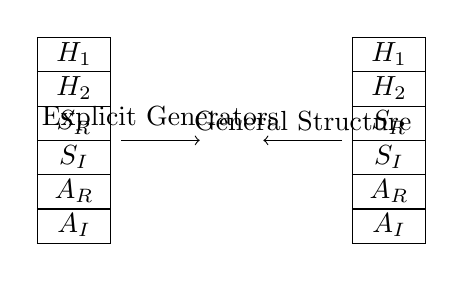
\begin{tikzpicture}[node distance=3cm]

\node (su4) at (0,0) {
    \begin{tabular}{|c|}
        \hline
        $H_1$ \\
        \hline
        $H_2$ \\
        \hline
        $S_R$ \\
        \hline
        $S_I$ \\
        \hline
        $A_R$ \\
        \hline
        $A_I$ \\
        \hline
    \end{tabular}
};

\node (general) at (4,0) {
    \begin{tabular}{|c|}
        \hline
        $H_1$ \\
        \hline
        $H_2$ \\
        \hline
        $S_R$ \\
        \hline
        $S_I$ \\
        \hline
        $A_R$ \\
        \hline
        $A_I$ \\
        \hline
    \end{tabular}
};

\draw[->] (su4.east) -- node[above] {Explicit Generators} ++(1,0);
\draw[->] (general.west) -- node[above] {General Structure} ++(-1,0);

\end{tikzpicture}

\end{document}